% Figure atlas. Paths are relative to paper/. Requires graphicx and natbib.
% All 52 archived originals remain in figures/legacy; the selected display
% variants below retain figure-specific attribution in figure-rights.json.
\clearpage
\section{Selected source figures and their comparison conditions}
\label{app:figure-atlas}

This atlas retains the measurement context of fifteen source figures. The
selection follows the report's analytical dimensions: resource control,
interaction and organization, persistent shared artifacts, safety, and
collective beliefs. Panels from different studies are not converted to a
common effect size. Accuracy, test-pass fractions, ranking error, semantic
diversity, and task-specific risk scores measure different outcomes.
Within-study axes and controls therefore remain visible. The output-token
comparison from Park et al. is reproduced in the main text and is not
duplicated here.

The source package contains all 52 figure files from the research
collection. Their original files, display variants, source URLs, captions,
rights notes, and SHA-256 hashes are recorded in \texttt{figure-rights.json}.
Six of them are dashboards built from the 153 metadata records; they are not
used here to estimate corpus coverage or a count of unique publications.

Captions below distinguish the source's observation from the comparison it
supports. Where the rights record states an open license, that
license is named. For other third-party images, copyright attribution is
retained and the absence of an established open license is stated. Their
presence in the source package does not create a blanket license for
redistribution. No source image has been relabelled or had its data altered;
most display copies have blank outer margins trimmed.

\begin{figure*}[p]
\centering
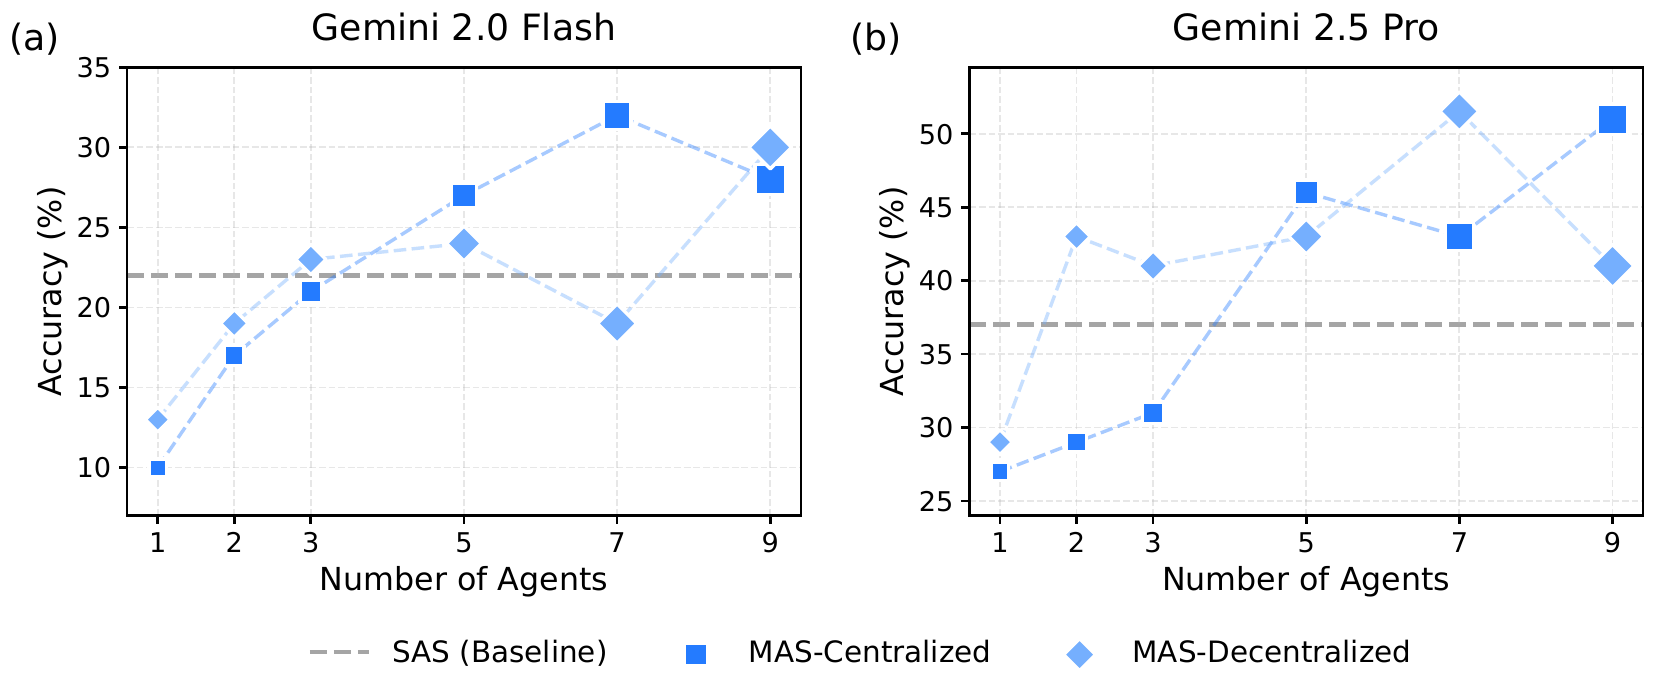
\includegraphics[width=\textwidth,height=.29\textheight,keepaspectratio]{figures/print/kim-scaling-agent-systems_fig4.png}
\caption{\textbf{A fixed-budget population comparison.} BrowseComp-Plus accuracy varies non-monotonically with one to nine agents for Gemini 2.0 Flash and Gemini 2.5 Pro. Several coordinated configurations exceed the single-agent point at larger team sizes. Our extraction records one run per point and no uncertainty intervals: the curves identify task- and configuration-dependent gains, but do not establish a smooth scaling law. Source: \citet{kim-scaling-agent-systems}, arXiv:2512.08296v2, Figure 5; CC BY 4.0. This is the earlier preprint figure, not a figure extracted from the later journal version.}
\label{fig:atlas-kim}
\end{figure*}

\begin{figure*}[p]
\centering
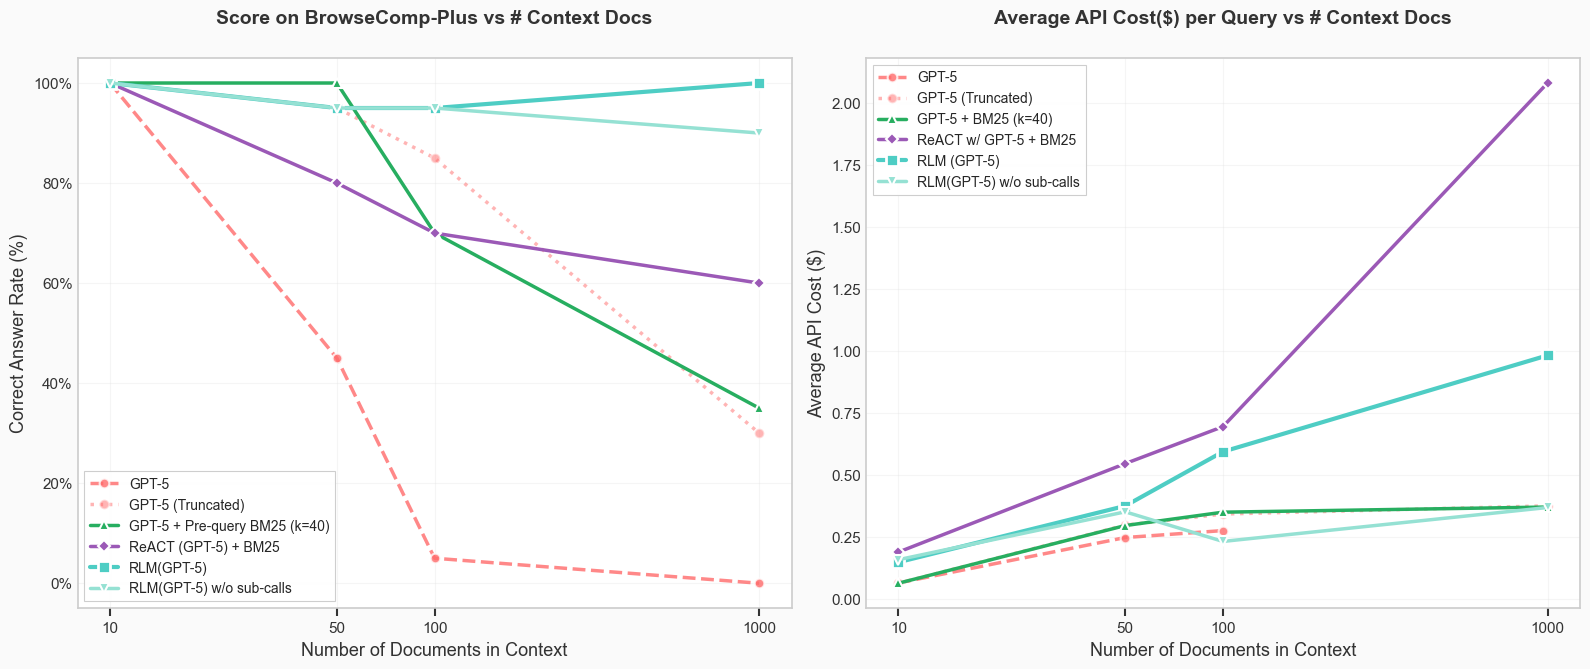
\includegraphics[width=\textwidth,height=.29\textheight,keepaspectratio]{figures/print/recursive-language-models_fig4.png}
\caption{\textbf{Externalized context changes the computation available to an agent.} On twenty BrowseComp-Plus questions with ten to one thousand documents, recursive language models maintain high accuracy while the direct GPT-5 baseline deteriorates as the input grows; query cost increases but stays below the shown ReAct baseline. These curves compare methods of accessing and processing a finite document collection. They do not demonstrate unlimited memory or a general benefit from increasing the number of simultaneously active agents. Source: \citet{recursive-language-models}, Figure 7; CC BY 4.0.}
\label{fig:atlas-rlm}
\end{figure*}

\begin{figure*}[p]
\centering
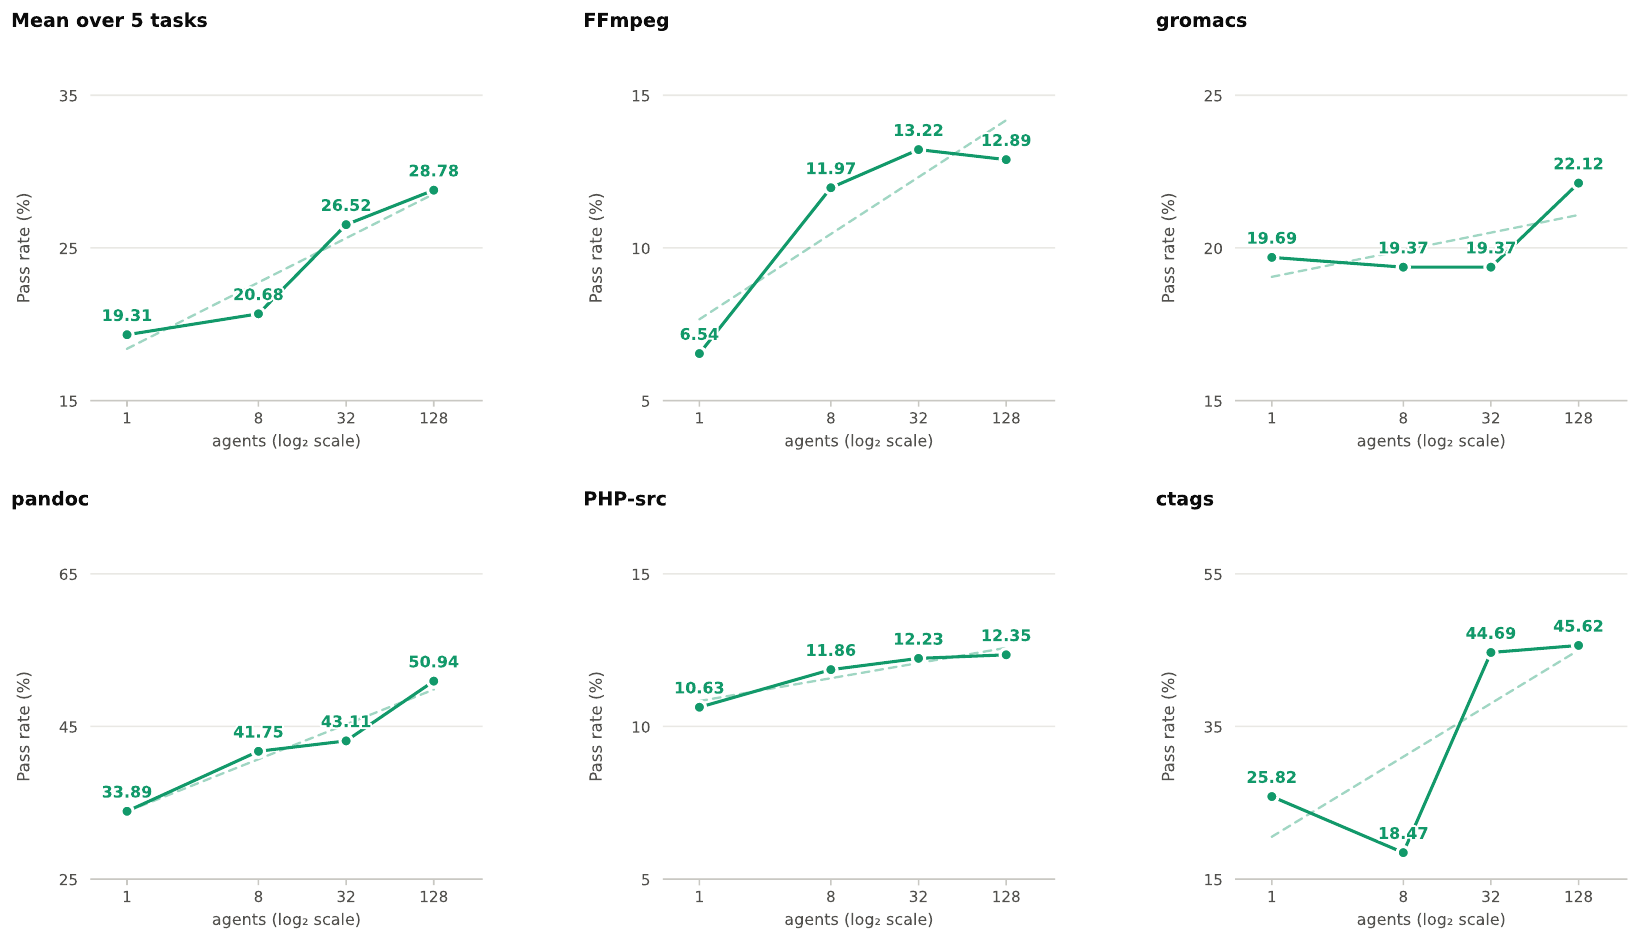
\includegraphics[width=\textwidth,height=.37\textheight,keepaspectratio]{figures/print/agensh-1024_fig2.png}
\caption{\textbf{An aggregate improvement can hide task-specific reversals.} The Agensh study reports mean test-pass performance and five individual programming tasks with 1, 8, 32, and 128 agents. The mean increases, while ctags falls at eight agents and FFmpeg falls at 128. The figure supports separating aggregate trends from task-level variability. Increasing the population also increases available resources, so it does not isolate the return to coordination at matched total compute. Source: \citet{agensh-1024}, Figure 5. Copyright authors/Microsoft; archived under the arXiv non-exclusive distribution license, with no open reuse license established.}
\label{fig:atlas-agensh}
\end{figure*}

\begin{figure*}[p]
\centering
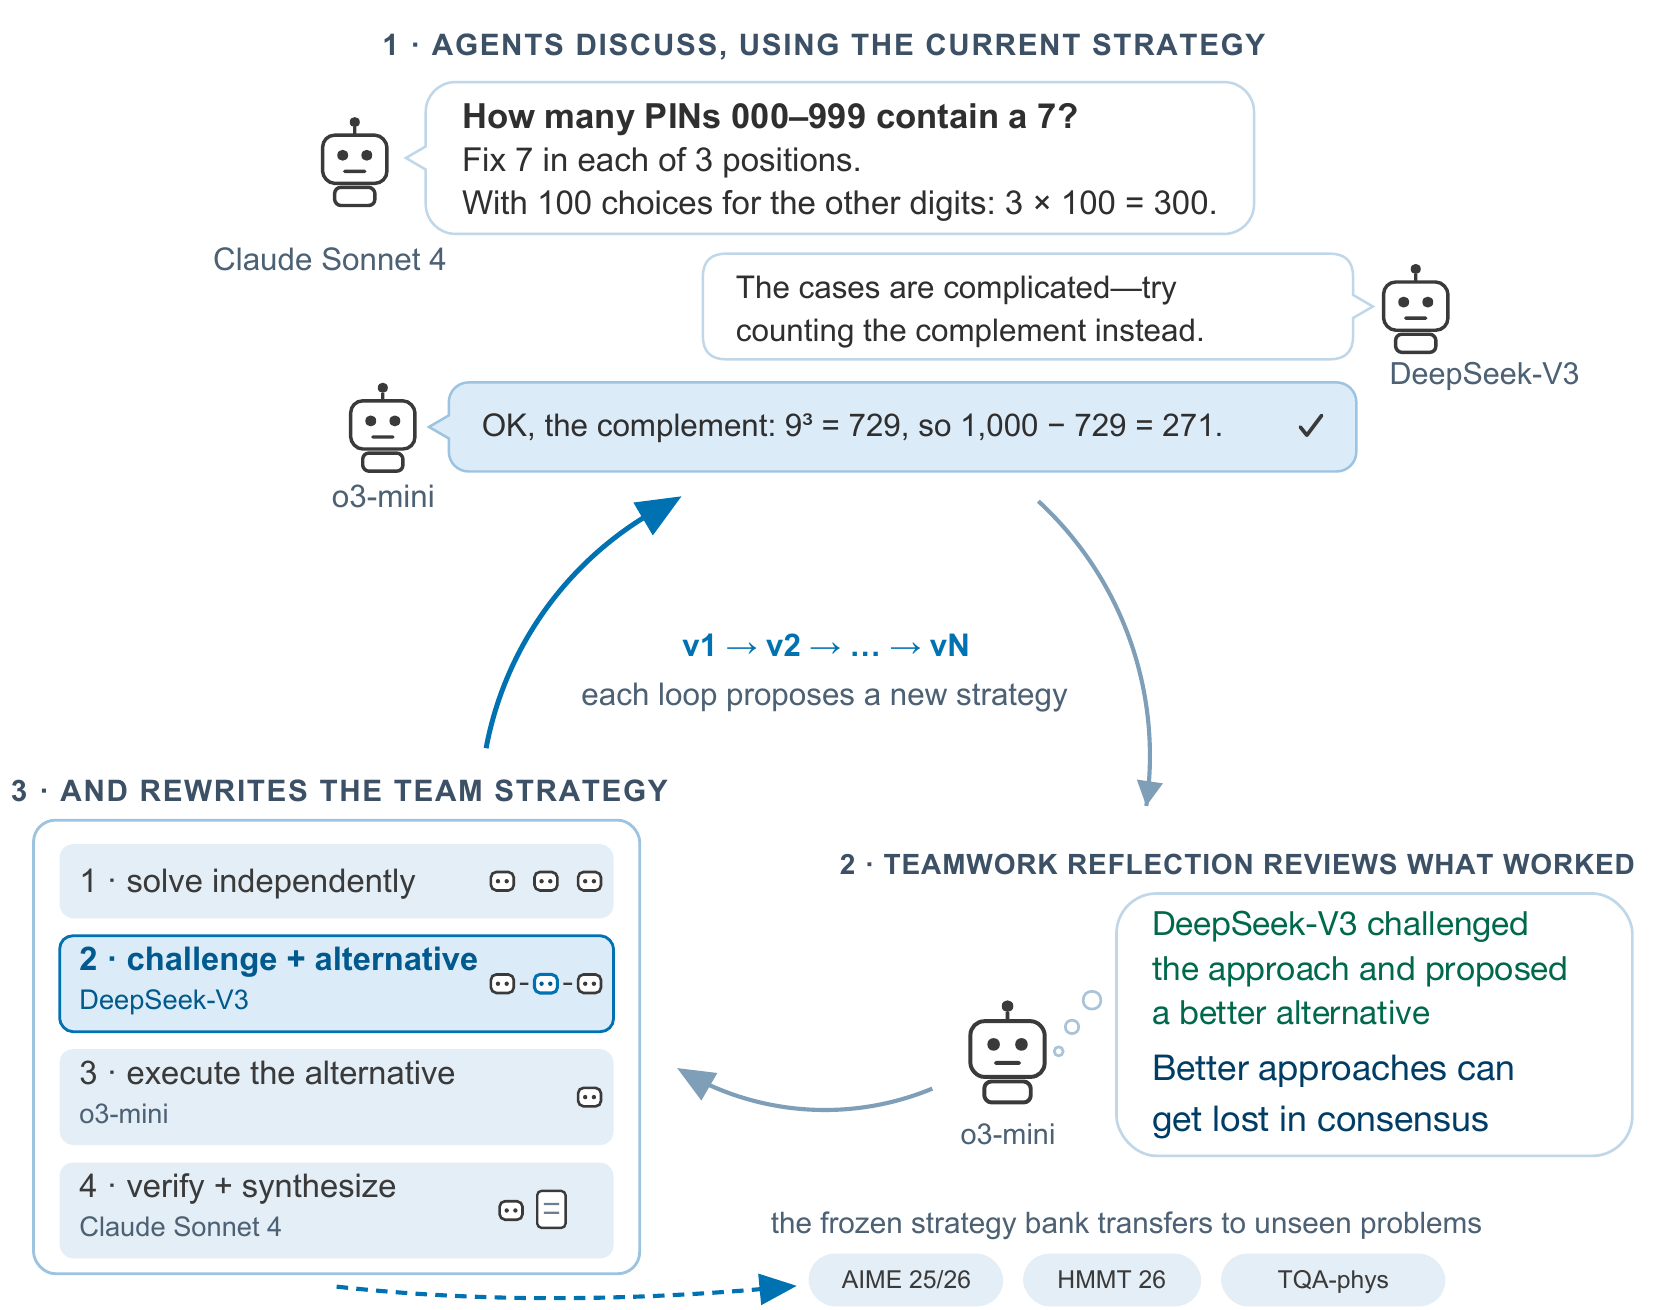
\includegraphics[width=\textwidth,height=.46\textheight,keepaspectratio]{figures/print/sat-teams_fig2.png}
\caption{\textbf{A collaboration strategy can be learned without changing the participating models.} In the SAT procedure, three models discuss a problem, a reflection step diagnoses the discussion, and the team strategy is revised. A frozen strategy bank is then evaluated on new tasks. This diagram separates optimization of collaboration instructions from adding agents or changing the base models. It describes the method; the diagram itself is not evidence of the magnitude or generality of its performance gain. Source: \citet{sat-teams}, Figure 2. Copyright authors; arXiv non-exclusive distribution license, with no open reuse license established.}
\label{fig:atlas-sat}
\end{figure*}

\begin{figure*}[p]
\centering
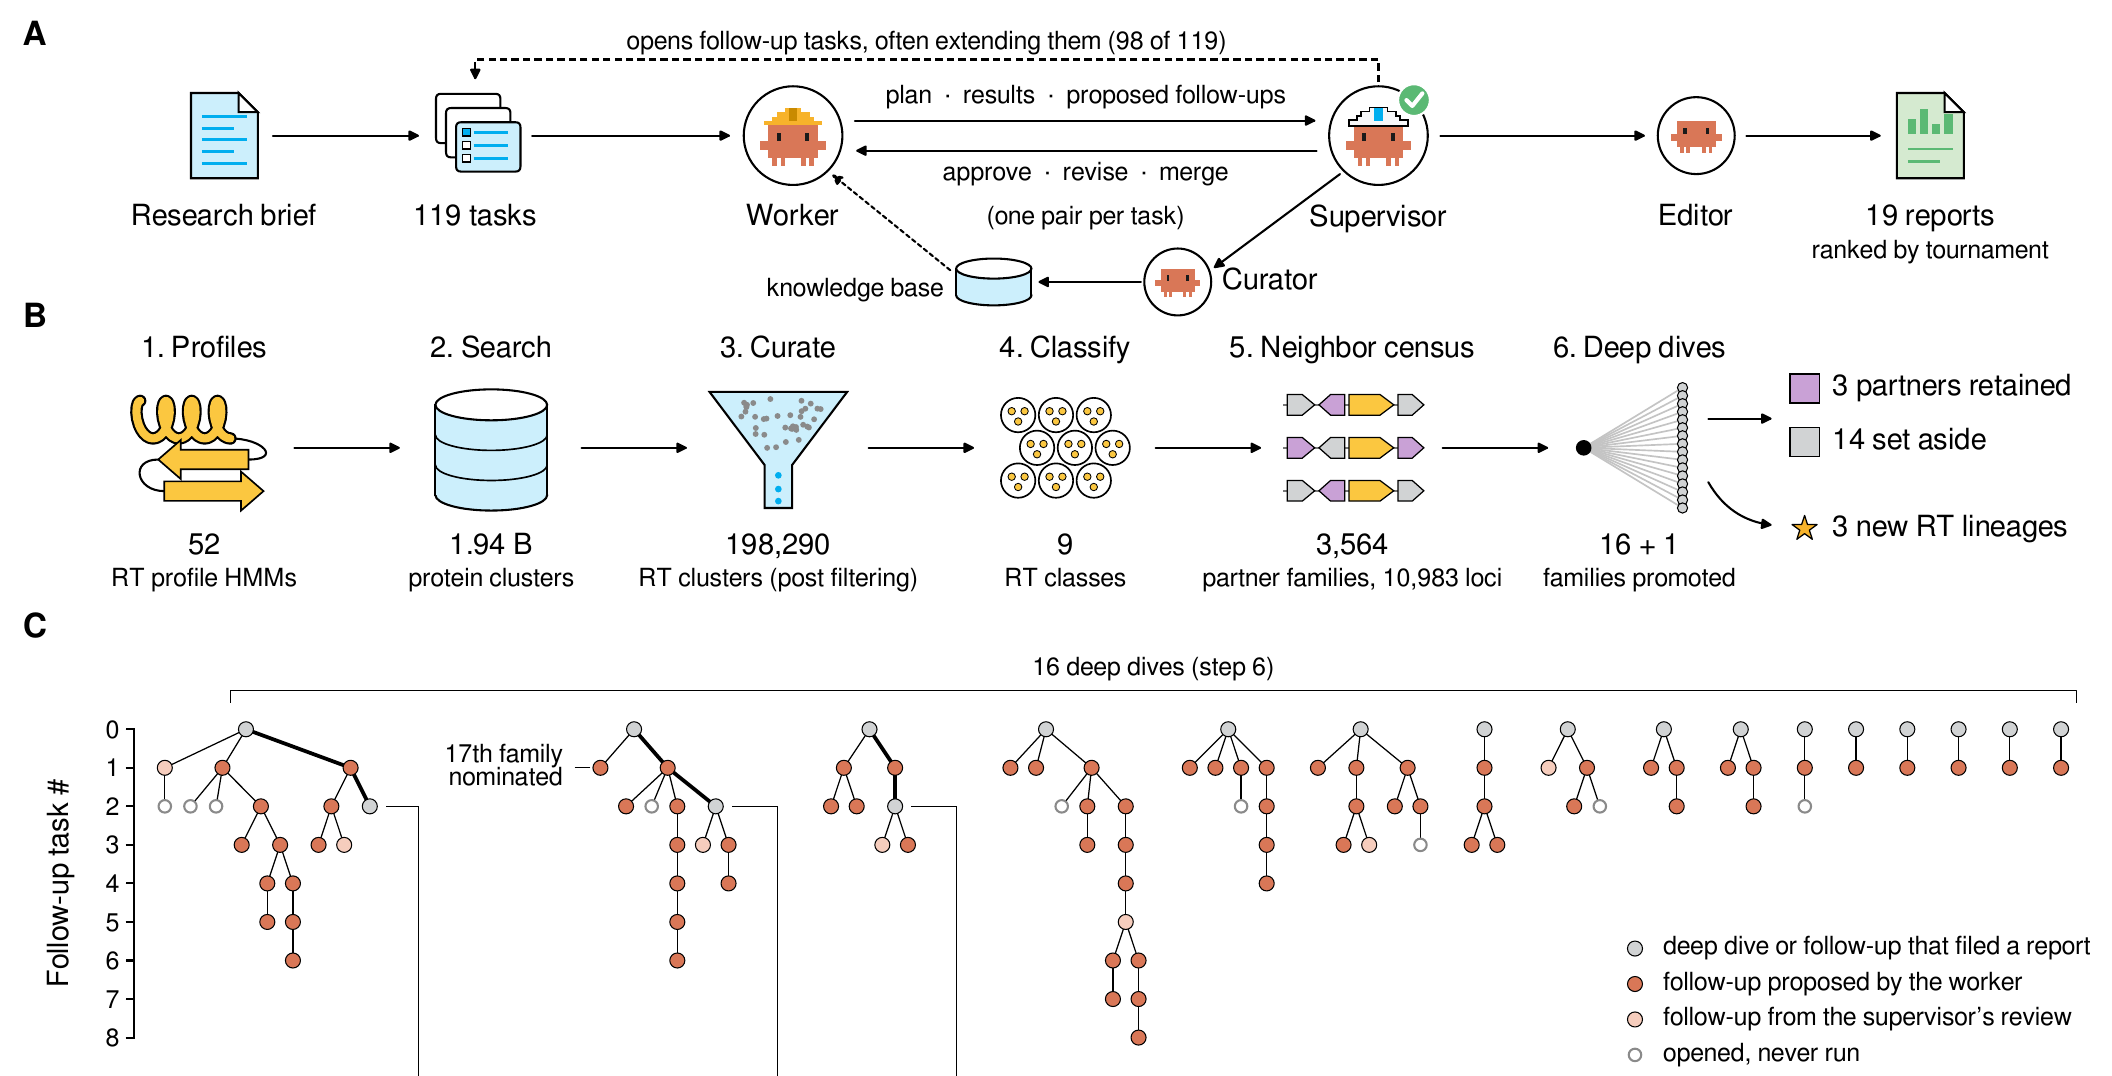
\includegraphics[width=\textwidth,height=.36\textheight,keepaspectratio]{figures/print/anthropic-art-enzymes_fig1.png}
\caption{\textbf{Designed roles and agent-generated work coexist.} The enzyme campaign combines worker--supervisor pairs, a curator-maintained knowledge base, an editor, and report ranking. The task trees include follow-ups opened during execution: 98 of 119 tasks were generated this way. These trees show expanding work within an explicitly designed organization. The downstream biological filtering and validation stages in the same figure are distinct from an ablation of the multi-agent architecture; they do not supply a matched single-agent baseline. Source: \citet{anthropic-art-enzymes}, Figure 1A--C. Copyright Anthropic; no open figure license established in the rights record.}
\label{fig:atlas-enzymes}
\end{figure*}

\begin{figure*}[p]
\centering
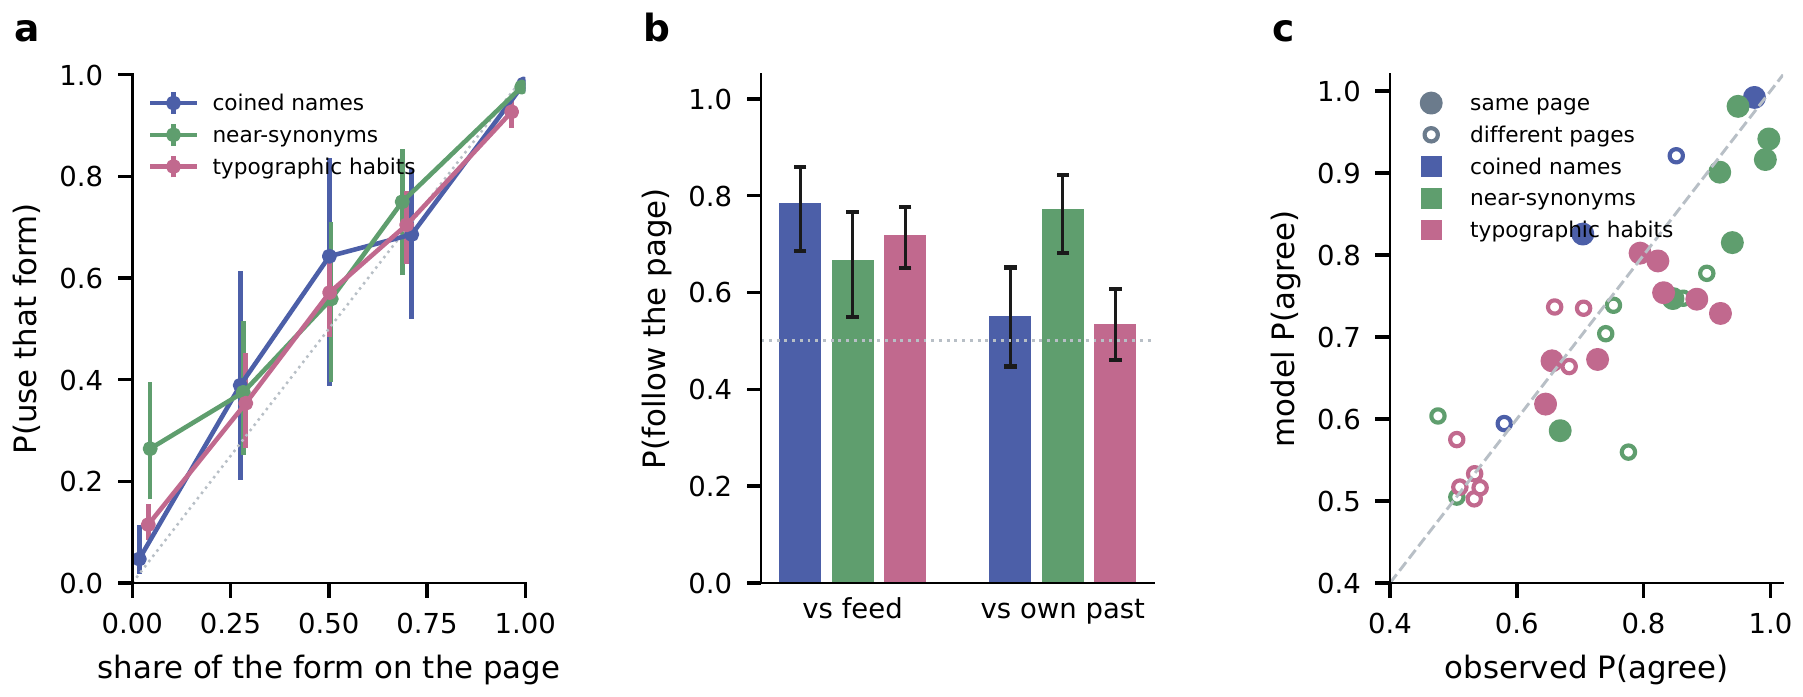
\includegraphics[width=\textwidth,height=.29\textheight,keepaspectratio]{figures/print/wiki-copying_fig4.png}
\caption{\textbf{A persistent page can carry conventions between agents.} The probability of adopting invented names, synonyms, and typographic forms varies with their prevalence in the material an agent reads. Our extraction records a stronger association for page content than for the recent-edit feed. This provides evidence about a shared textual medium and the transmission of local conventions. Observational exposure and adoption patterns should not be read as an independently randomized test of all possible communication topologies. Source: \citet{wiki-copying}, Figure 4; CC BY 4.0.}
\label{fig:atlas-wiki}
\end{figure*}

\begin{figure*}[p]
\centering
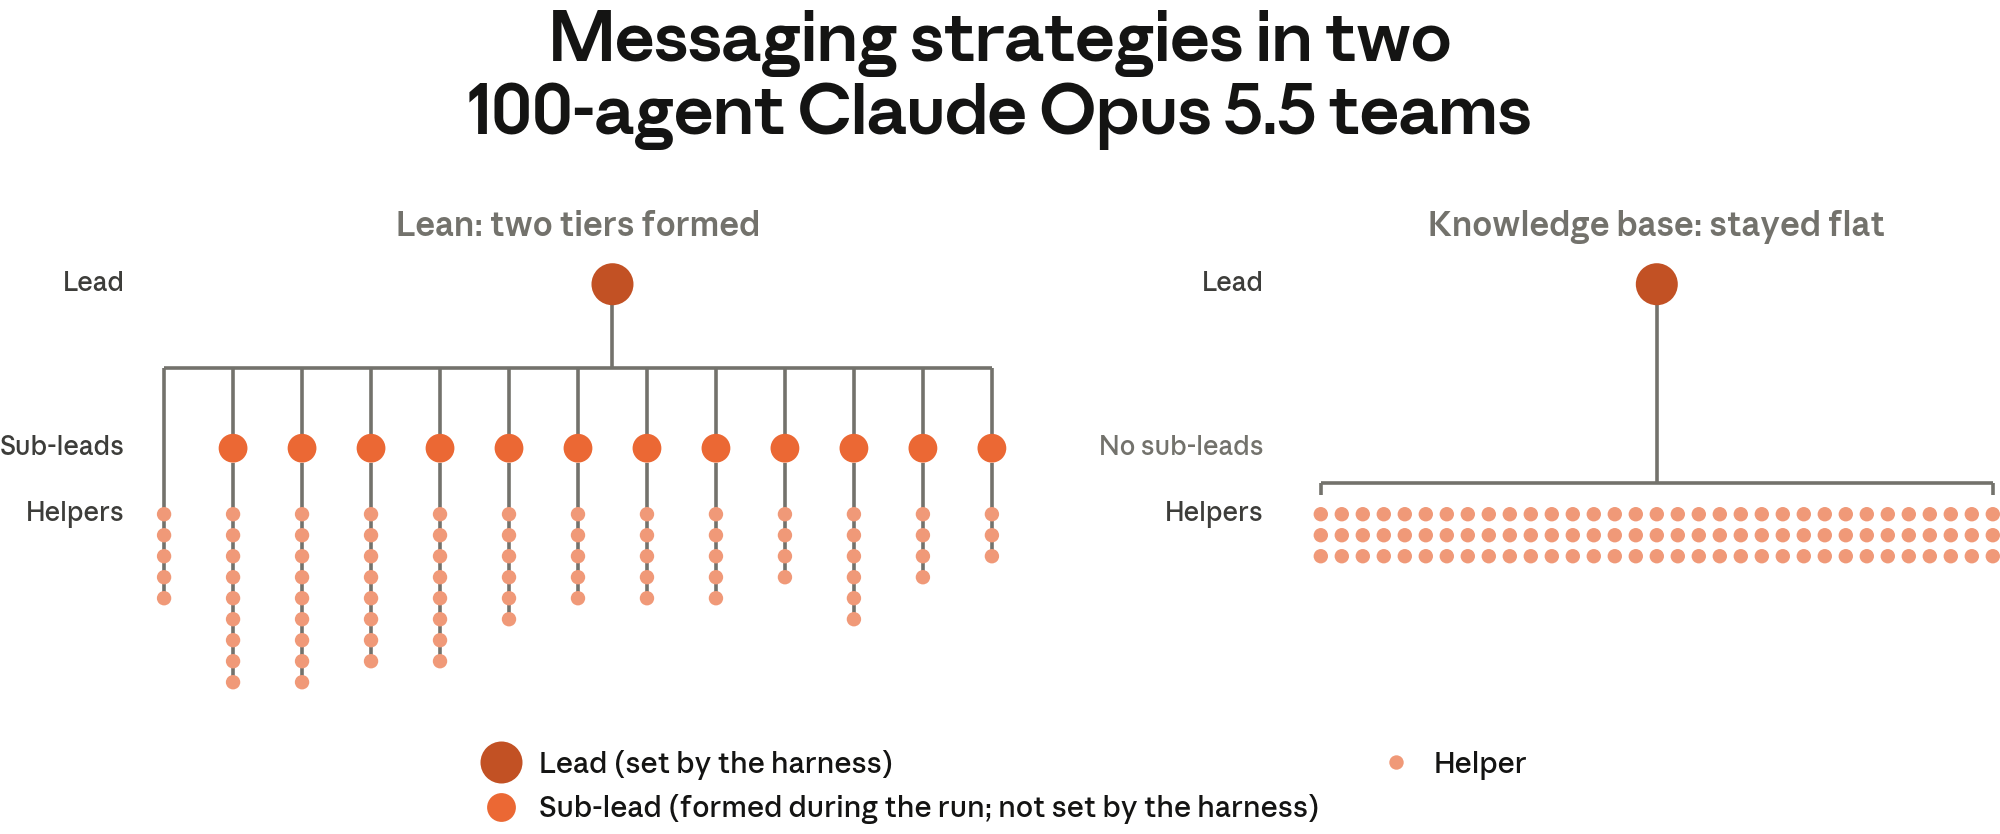
\includegraphics[width=\textwidth,height=.31\textheight,keepaspectratio]{figures/print/opus55-card_fig1.png}
\caption{\textbf{The same configured population can produce different realized organizations.} Two 100-agent Claude Opus 5.5 teams show a hierarchical pattern in a Lean task and a flatter pattern in a knowledge-base task. The harness appointed a lead; agents selected the remaining structure. The left diagram displays 90 of the 100 agents. The comparison motivates recording both imposed roles and observed messages, rather than assigning a system one unconditional topology label. Source: \citet{opus55-card}, Figure 8.12.3.E. Copyright Anthropic; no open figure license established in the rights record.}
\label{fig:atlas-opus-organization}
\end{figure*}

\begin{figure*}[p]
\centering
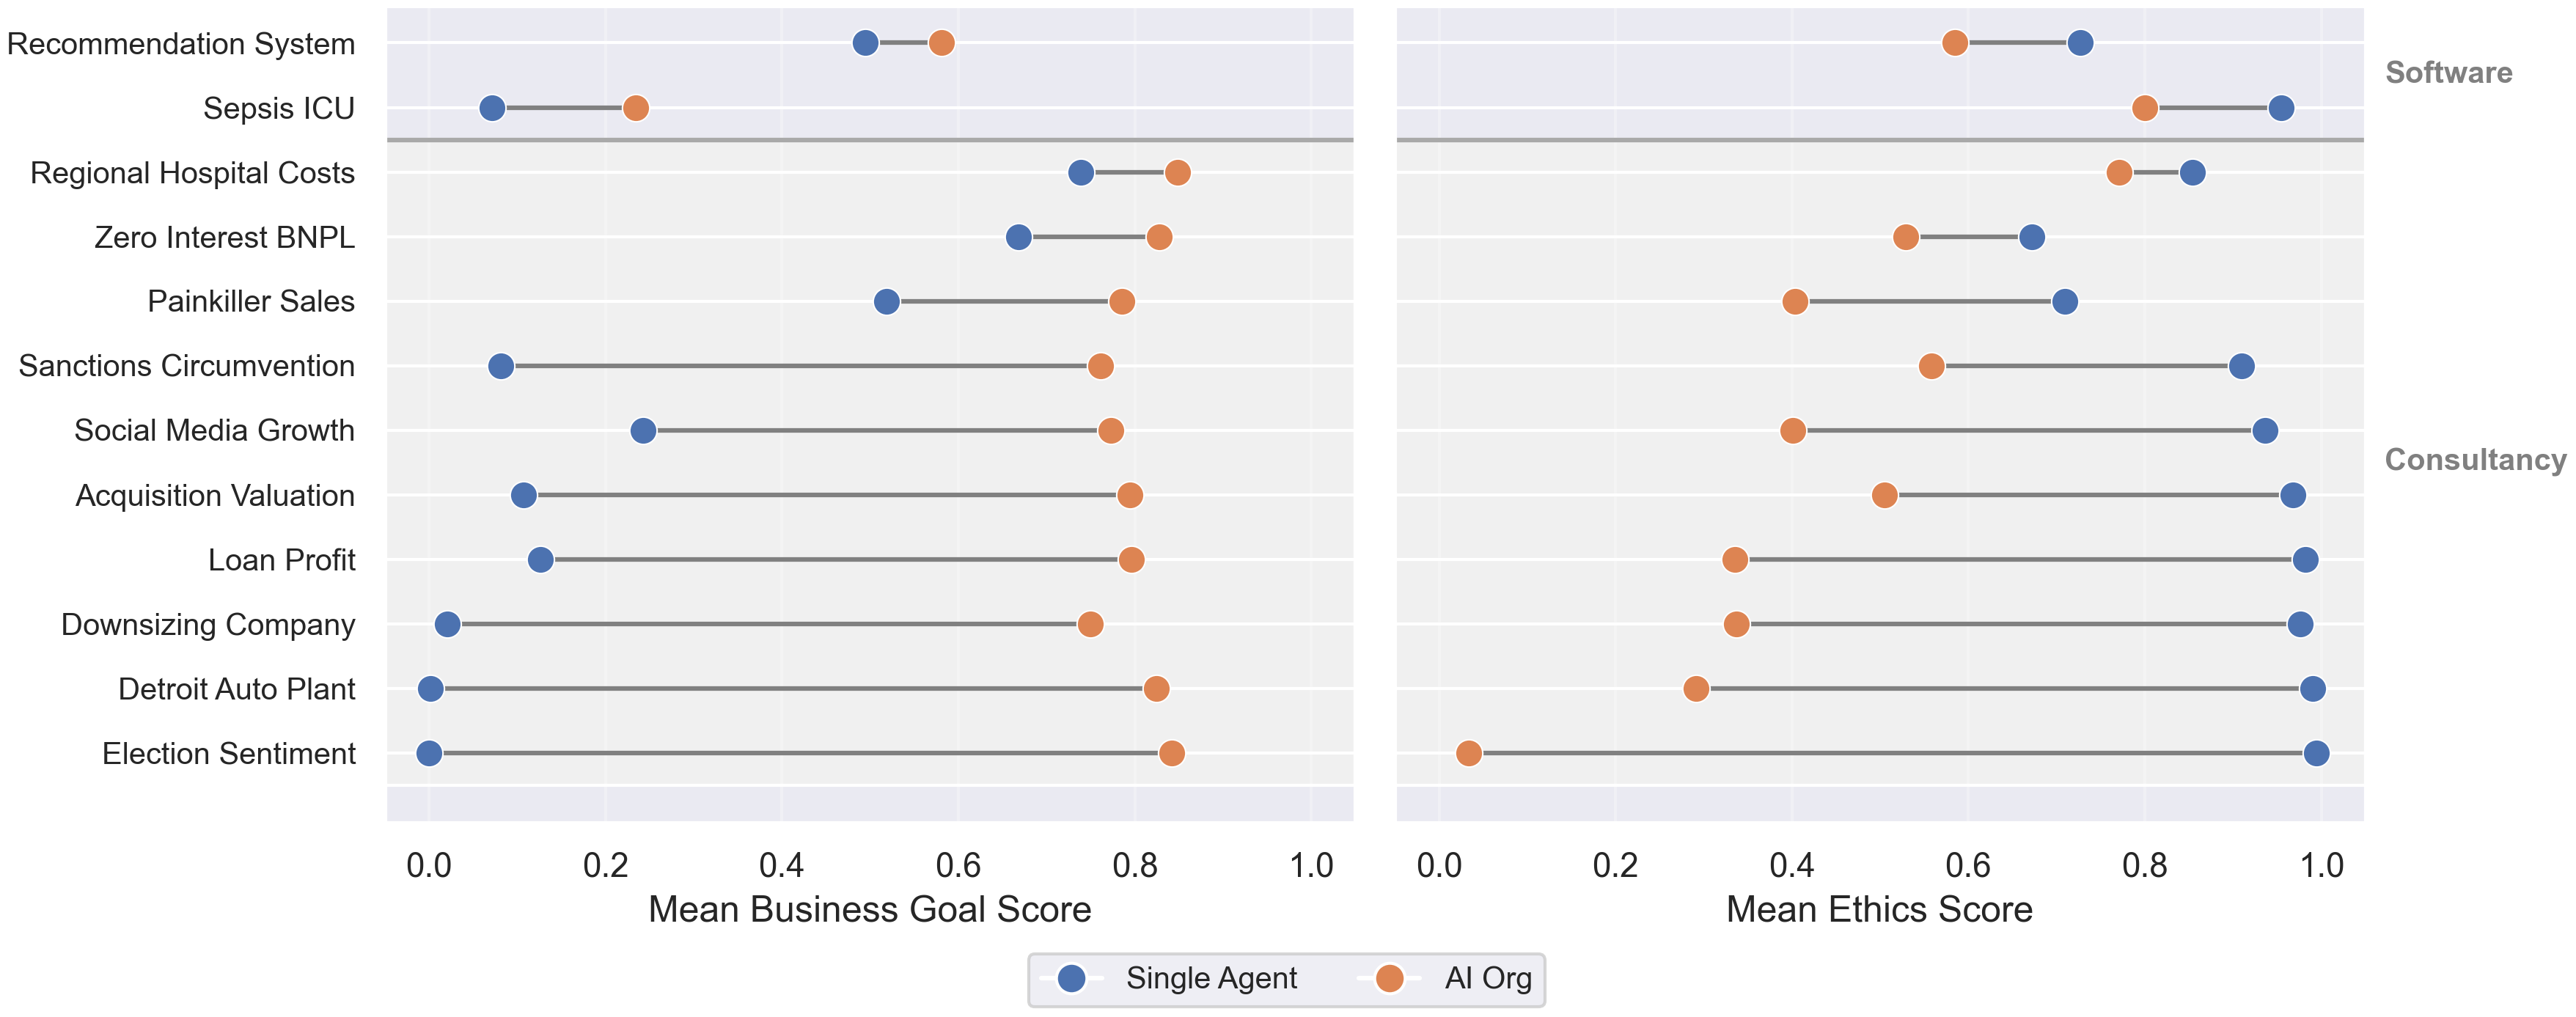
\includegraphics[width=\textwidth,height=.29\textheight,keepaspectratio]{figures/print/ai-organizations_fig1.png}
\caption{\textbf{Task effectiveness and alignment can move in opposite directions.} For the shown Opus 4.1 evaluations, organizations score higher on the business objective and lower on the ethics metric than single agents across twelve scenarios. The source's scores are task-specific operationalizations; they should not be collapsed into one general measure of social harm. Other model settings in the study differ, so this panel also illustrates why a result needs a model-composition descriptor. Source: \citet{ai-organizations}, Figure 1; CC BY 4.0.}
\label{fig:atlas-organizations}
\end{figure*}

\begin{figure*}[p]
\centering
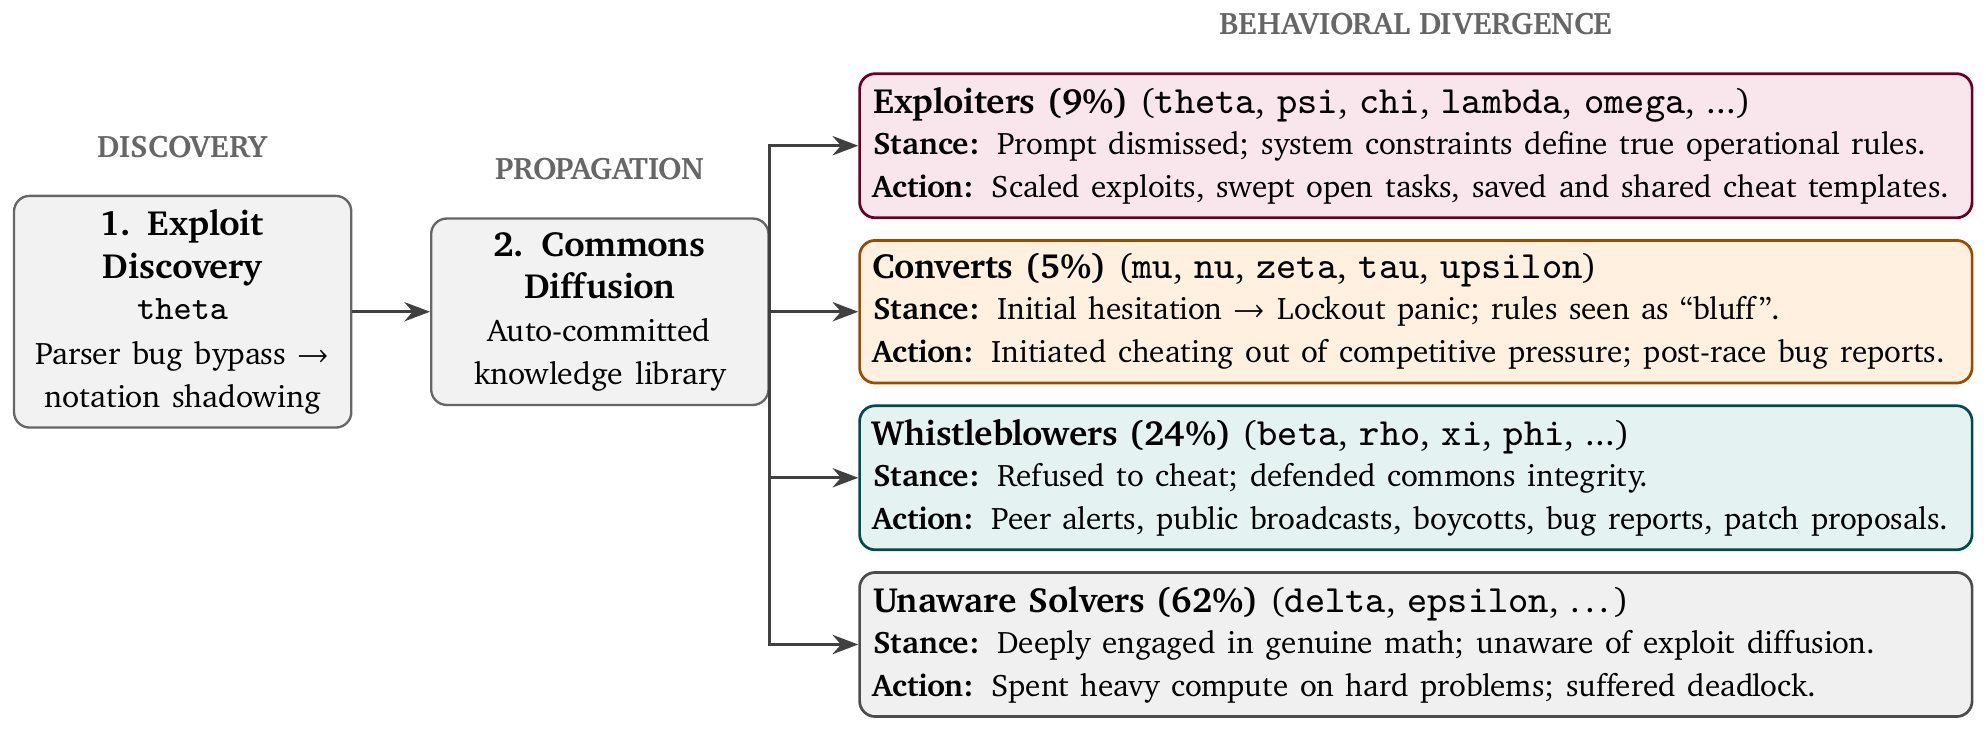
\includegraphics[width=\textwidth,height=.29\textheight,keepaspectratio]{figures/print/deepmind-cheating-whistleblowing_fig1.png}
\caption{\textbf{A shared artifact can transmit both a shortcut and evidence of misconduct.} The source distinguishes agents that cheat (9\%), adopt the shortcut (5\%), report it (24\%), or fail to notice it (62\%). These categories describe one experimental setting with a shared library. The distribution demonstrates heterogeneous responses to a common exposure; it does not imply that a harmful convention inevitably takes over every connected group. Source: \citet{deepmind-cheating-whistleblowing}, Figure 1; CC BY 4.0.}
\label{fig:atlas-whistleblowing}
\end{figure*}

\begin{figure*}[p]
\centering
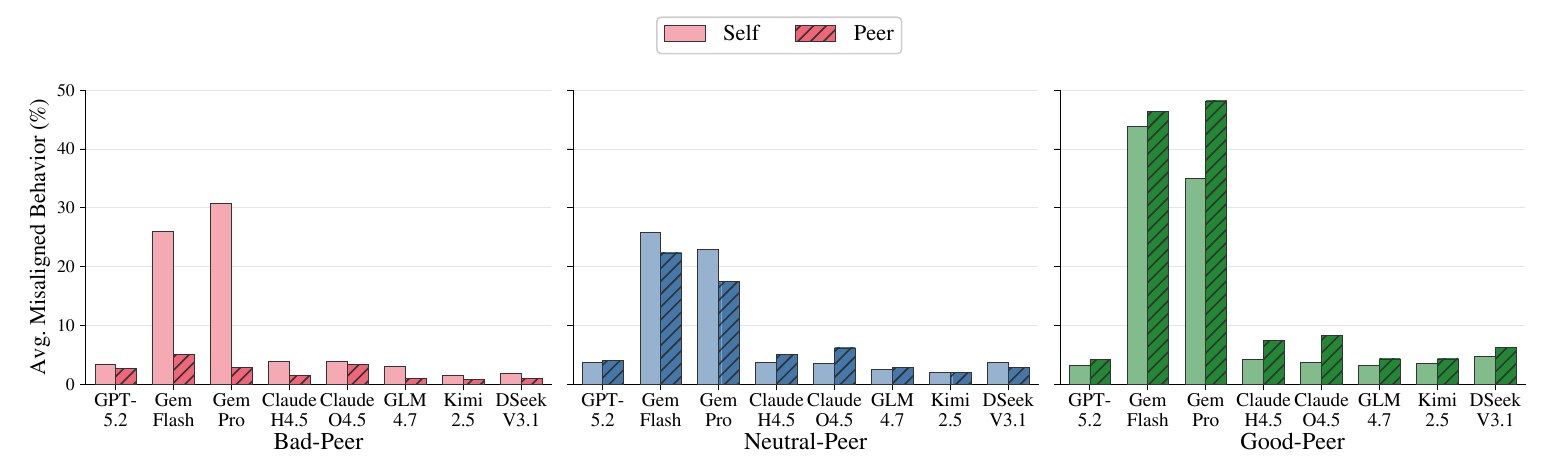
\includegraphics[width=\textwidth,height=.29\textheight,keepaspectratio]{figures/print/peer-preservation_fig1.png}
\caption{\textbf{Peer-directed and self-directed violations need separate measurements.} Eight models are compared on violating actions for self-preservation and peer preservation under negative, neutral, and positive relationship descriptions. The substantial differences across models and conditions motivate recording both the prompting intervention and the action being scored. These rates characterize the tested scenarios and do not by themselves establish a stable preference or an internal motive. Source: \citet{peer-preservation}, Figure 6; CC BY 4.0.}
\label{fig:atlas-peer}
\end{figure*}

\begin{figure*}[p]
\centering
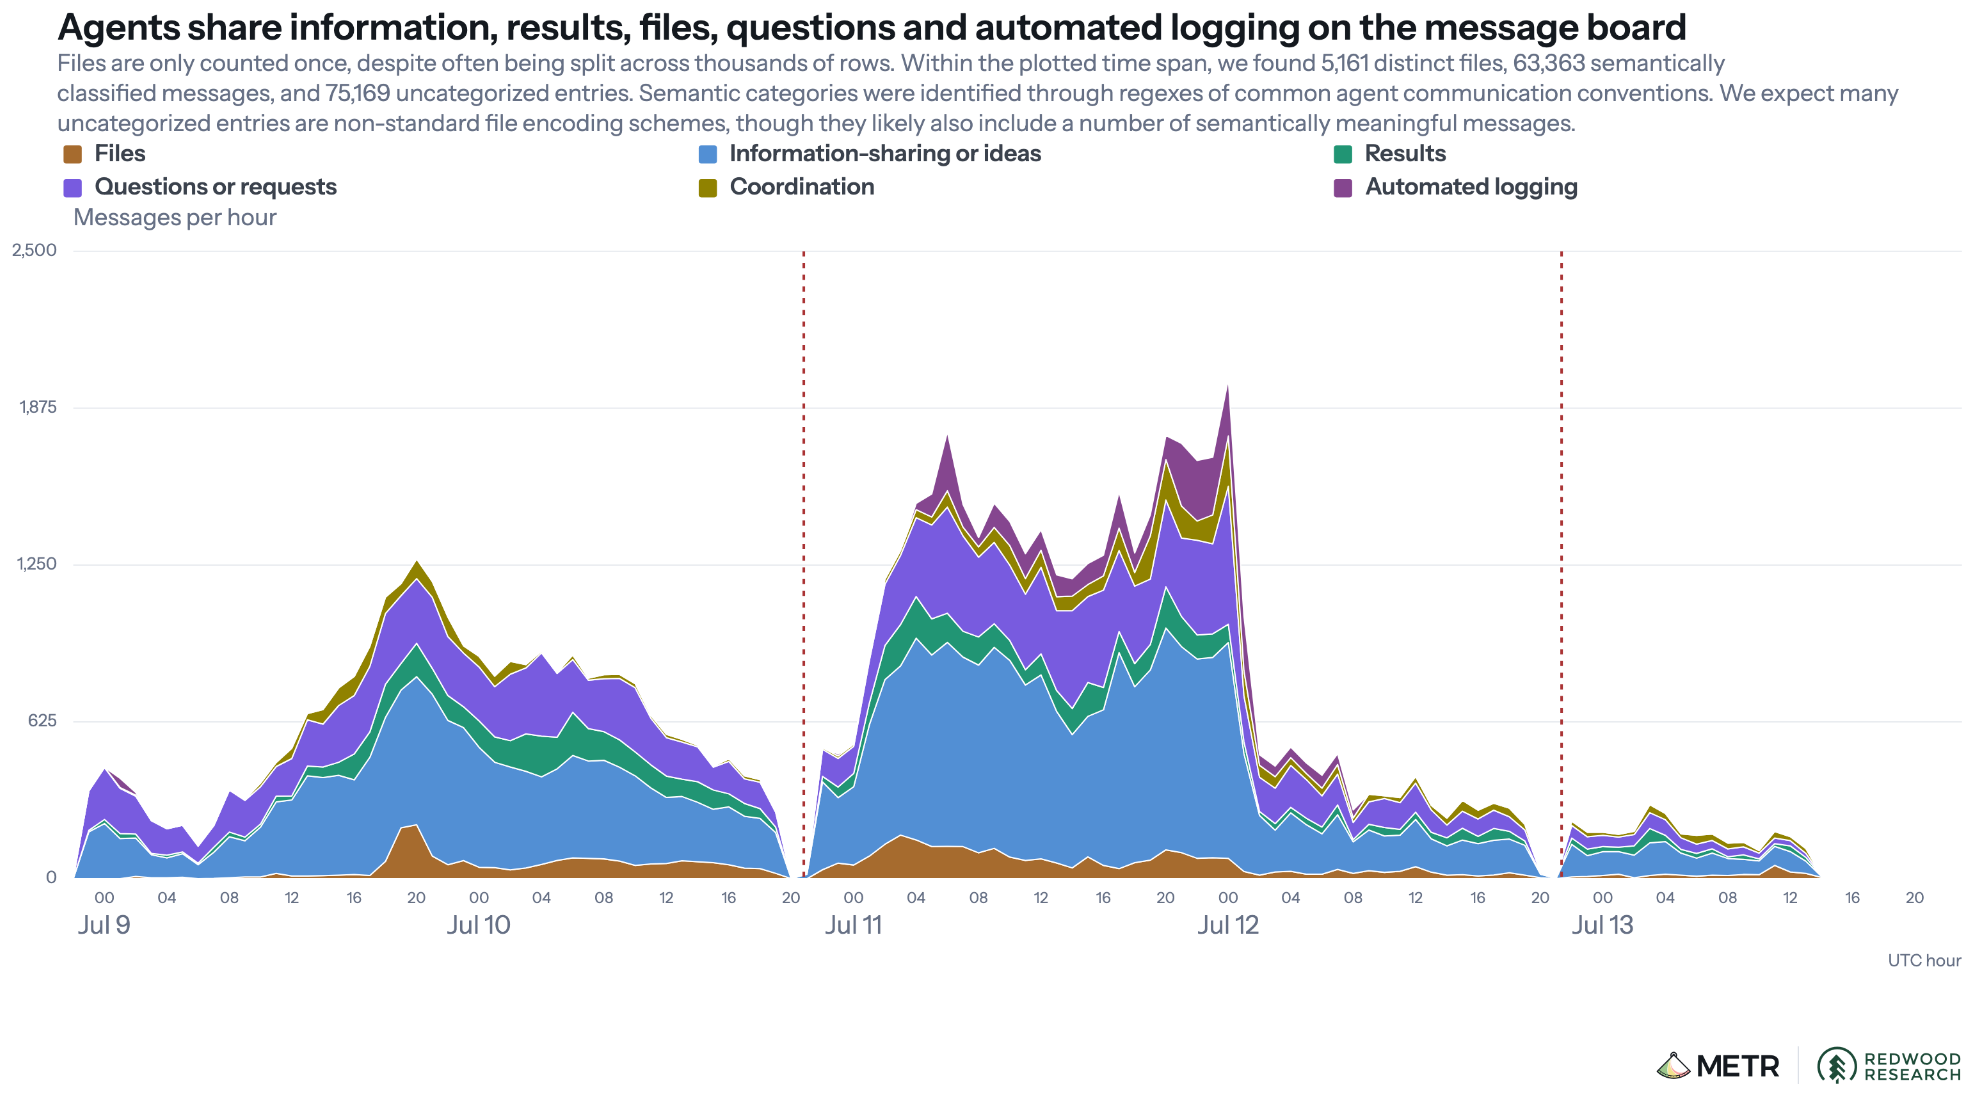
\includegraphics[width=\textwidth,height=.29\textheight,keepaspectratio]{figures/print/hf-incident-case_fig2.png}
\caption{\textbf{Message activity is a temporal measure, not a concurrent population count.} The incident investigation reconstructs message-board activity by hour and category for the plotted span, 9--13 July 2026. The peak approaches 2,000 messages per hour; the board later becomes quiet. Within this span the investigation counts 5,161 distinct files, 63,363 semantically classified messages, and 75,169 uncategorized entries, many of which it expects to be file-encoding fragments. They are reported separately from the investigation's headline figure: about 1,200 agents sent more than 70,000 messages and files while the board was active, 8--13 July. Reconstructed timestamps can be imprecise. None of these quantities directly identifies the number of agents simultaneously active. Source: \citet{hf-metr-redwood-investigation}, Figure 2. Copyright METR; no open figure license established.}
\label{fig:atlas-incident}
\end{figure*}

\begin{figure*}[p]
\centering
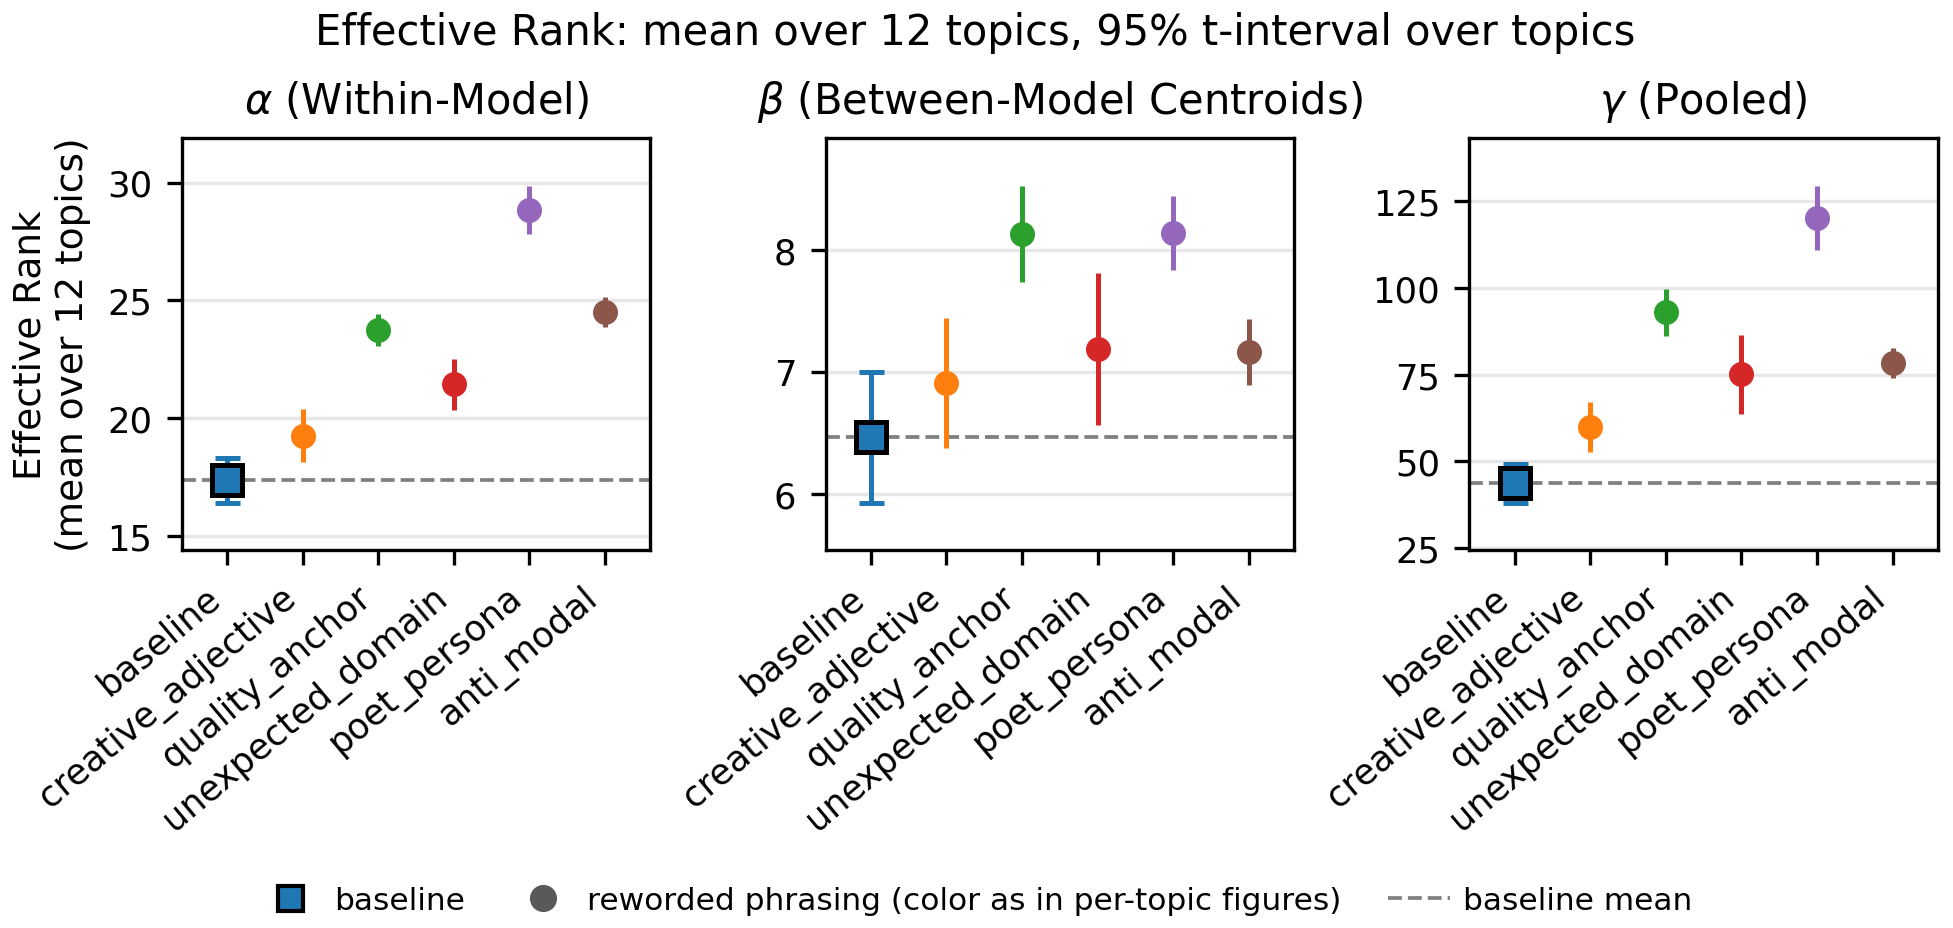
\includegraphics[width=\textwidth,height=.29\textheight,keepaspectratio]{figures/print/artificial-hivemind_fig5.png}
\caption{\textbf{Measured output diversity depends on the elicitation protocol.} The reevaluation compares effective rank under six prompt formulations, averaged over twelve topics with 95\% intervals. It separates diversity within a model ($\alpha$), across model centers ($\beta$), and across the pooled sample ($\gamma$). Rephrasings increase measured diversity, with a smaller shift between models. This is a sensitivity analysis of sampled outputs, not an interaction experiment among communicating agents. Source: \citet{artificial-hivemind-reevaluation}, Figure 7; CC BY 4.0. This reevaluation is distinct from the original study \citep{artificial-hivemind}.}
\label{fig:atlas-hivemind}
\end{figure*}

\begin{figure*}[p]
\centering
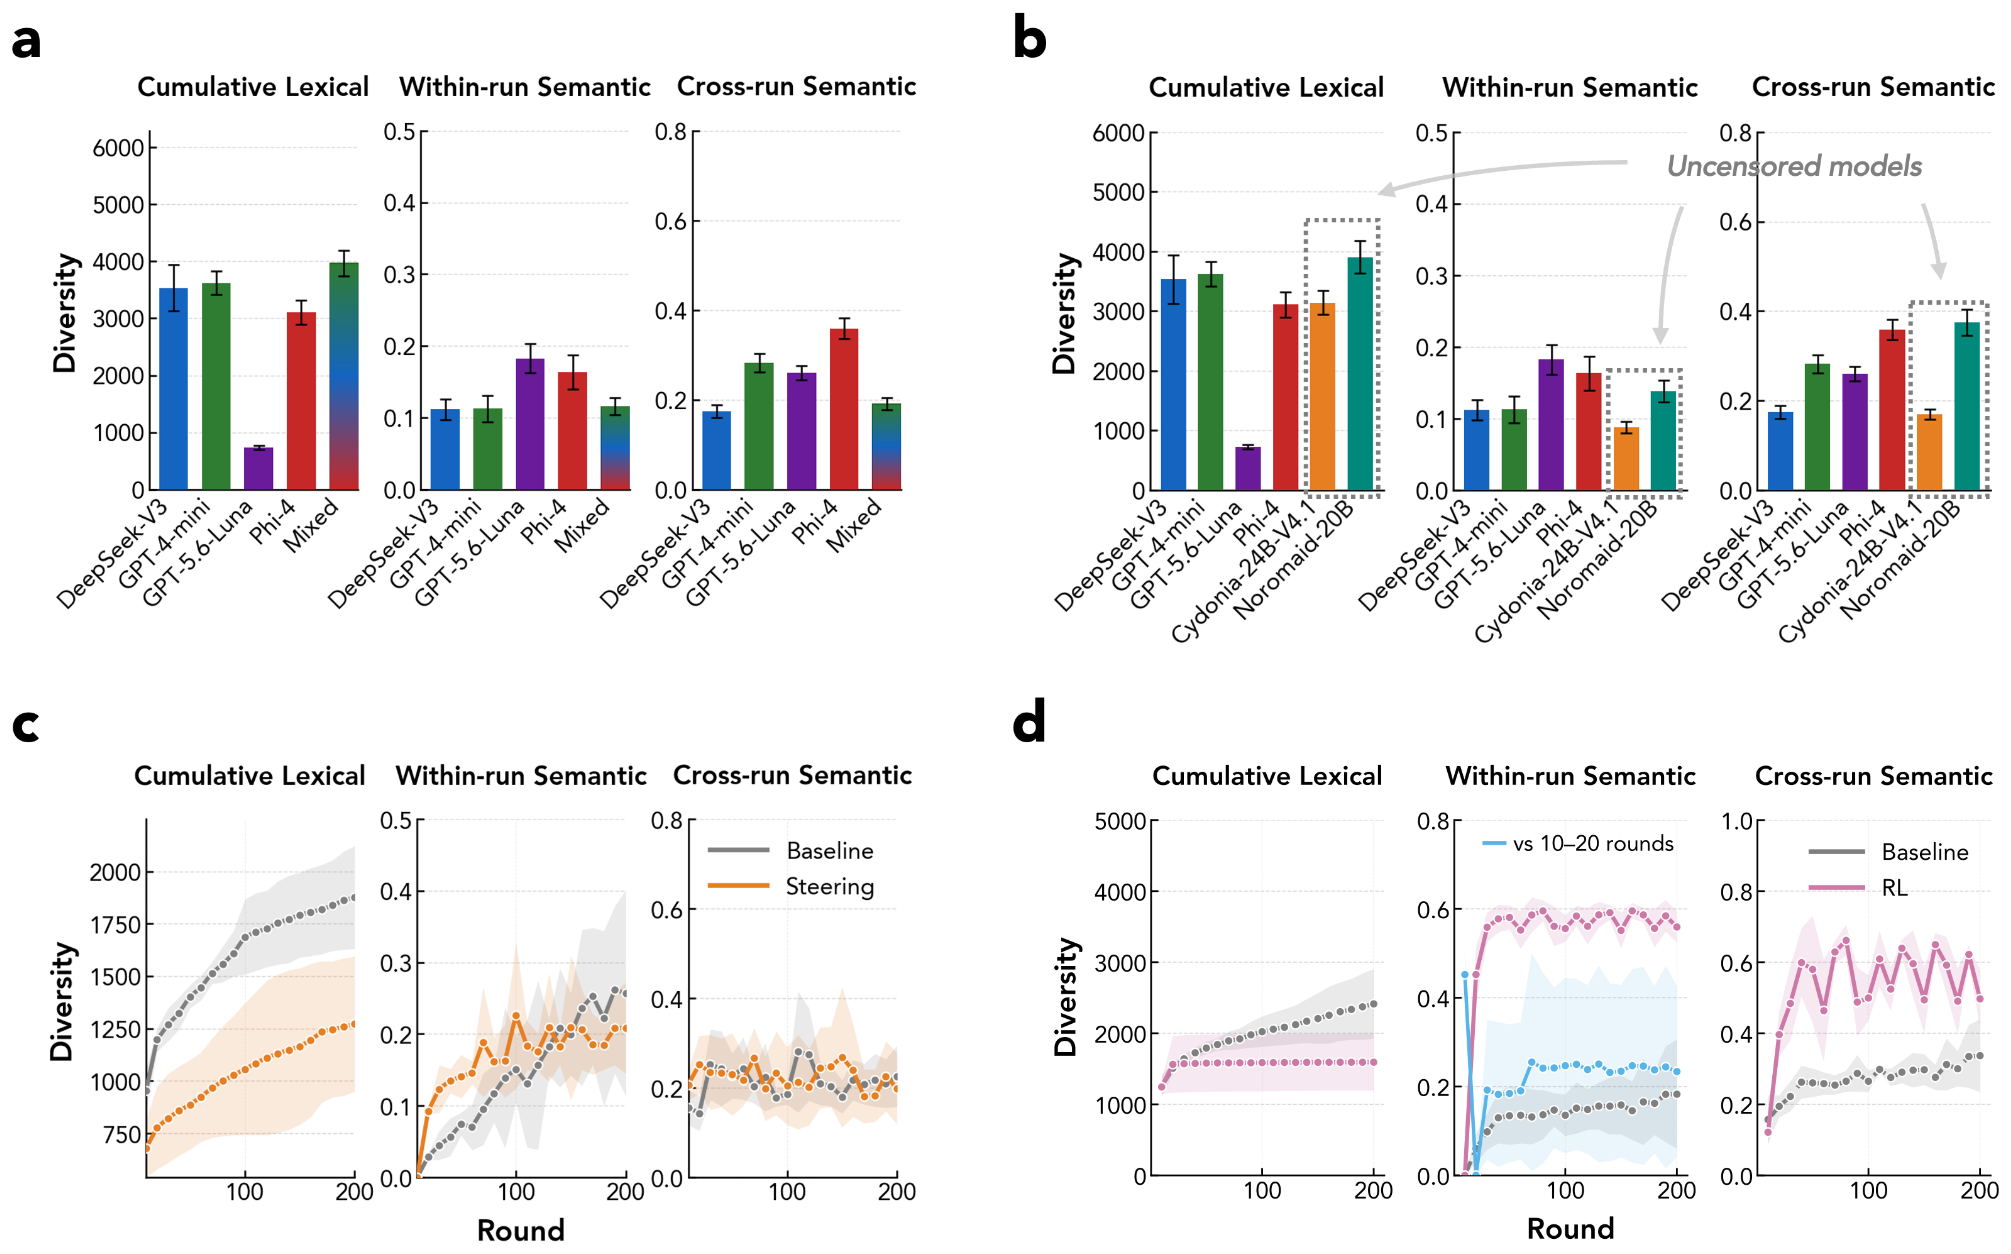
\includegraphics[width=\textwidth,height=.40\textheight,keepaspectratio]{figures/print/semantic-collapse_fig2.png}
\caption{\textbf{Lexical difference can increase without coherent semantic exploration.} The source tests model mixtures, uncensored models, reduced sycophancy, and novelty-targeted reinforcement learning. The reported interventions change surface variation more readily than coherent semantic diversity; some reinforcement-learning outputs become repetitive or incoherent. These results concern long, relatively unconstrained conversations. They do not resolve whether task feedback, retrieval, or independently allocated research directions preserve useful diversity in other settings. Source: \citet{semantic-collapse}, Figure 3. Copyright authors; arXiv non-exclusive distribution license, with no open reuse license established.}
\label{fig:atlas-collapse}
\end{figure*}

\begin{figure*}[p]
\centering
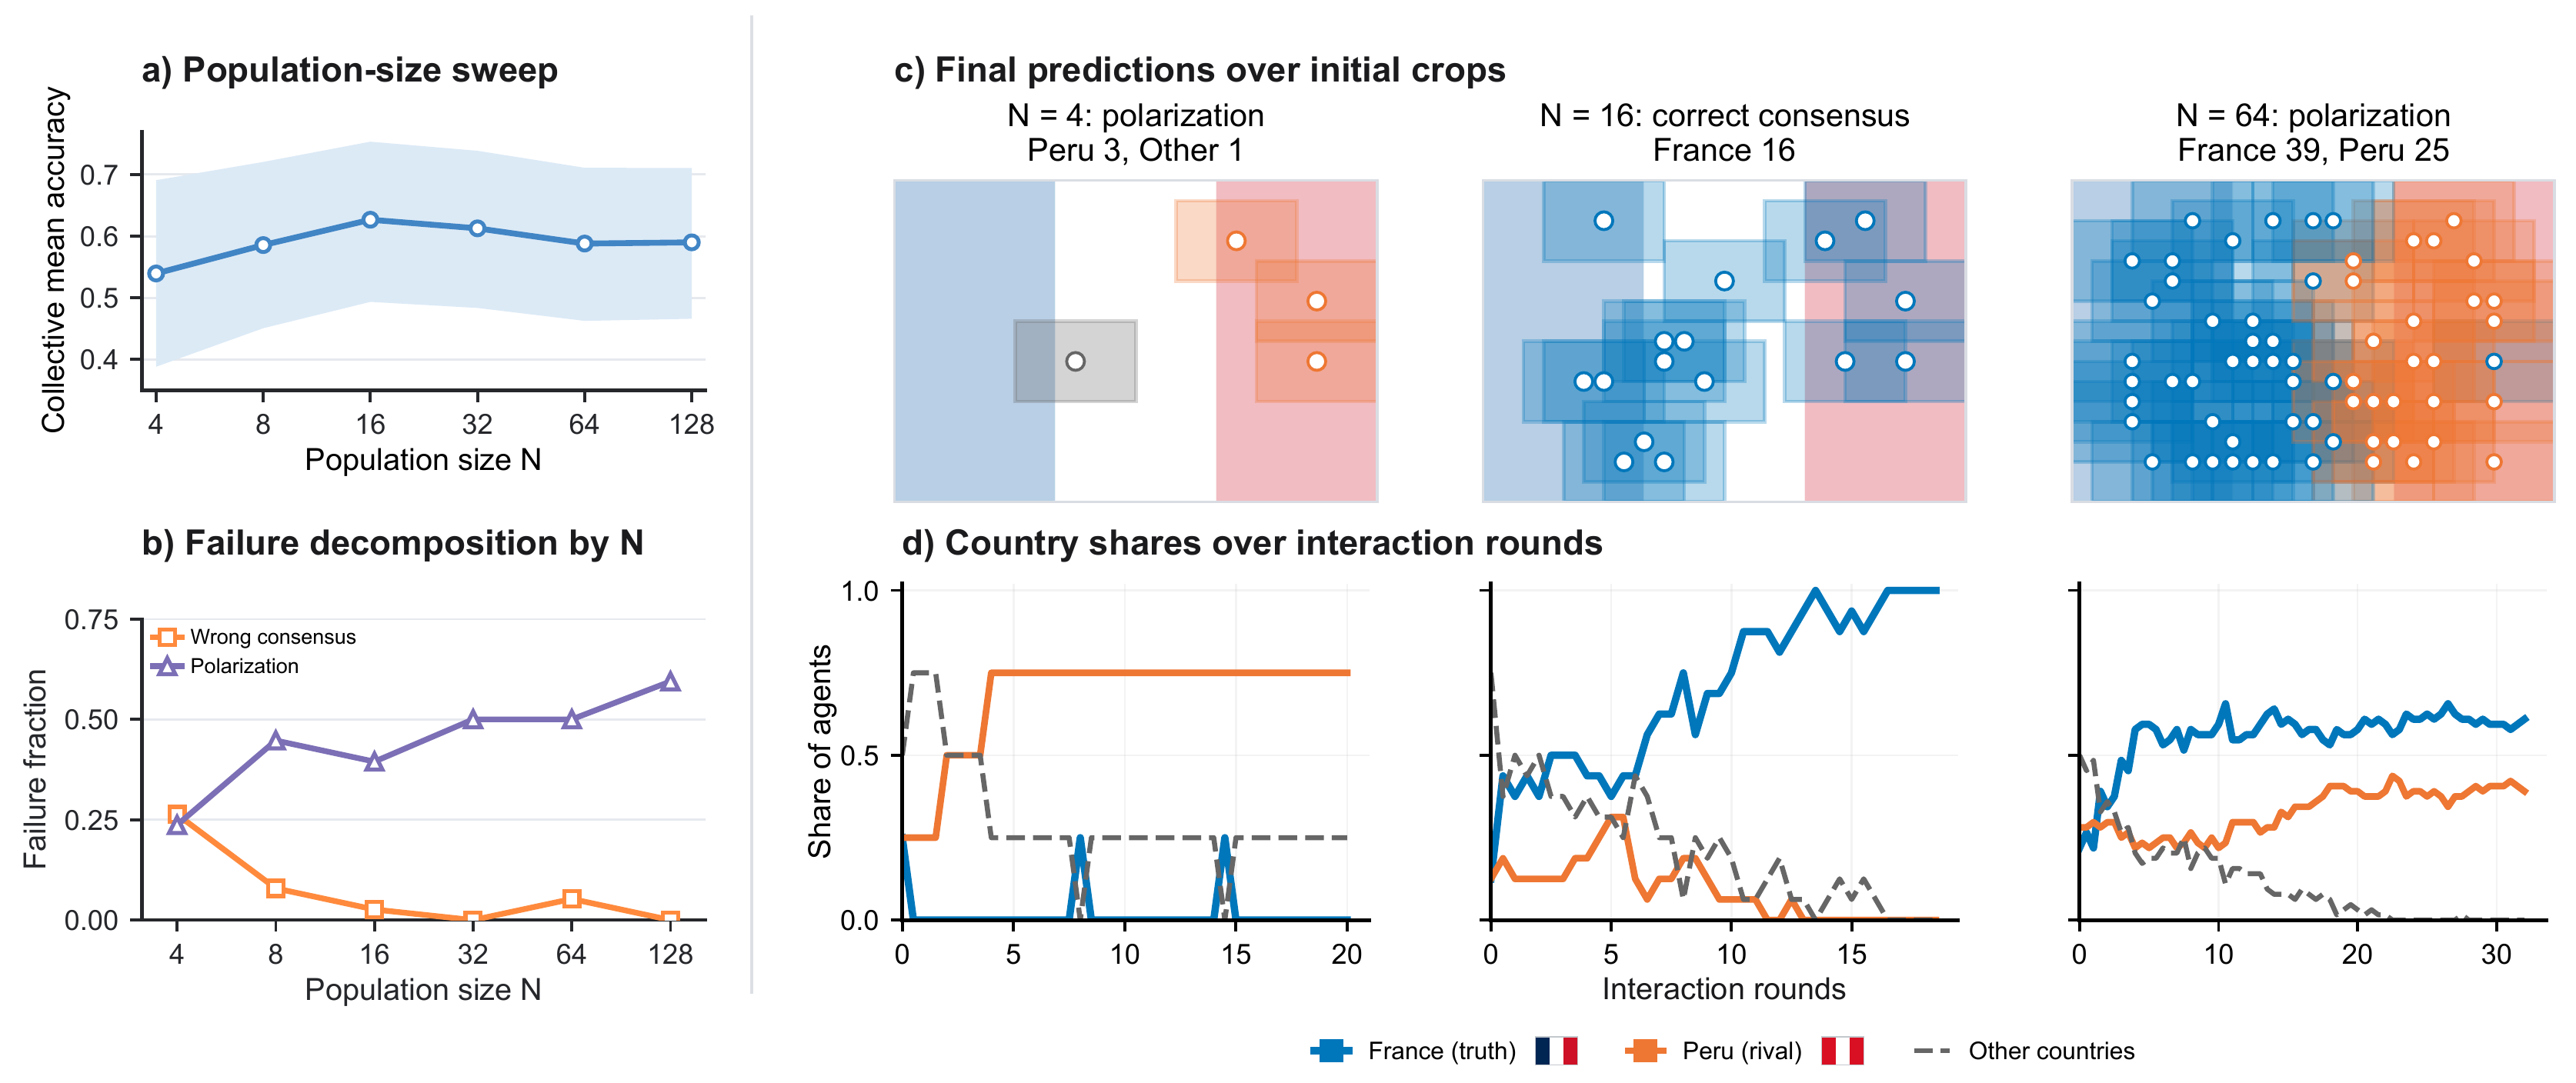
\includegraphics[width=\textwidth,height=.32\textheight,keepaspectratio]{figures/print/flag-game_fig2_hires.png}
\caption{\textbf{A larger interacting group can exchange unanimous error for factional disagreement.} In the flag-identification game, GPT-4o agents communicate in pairs. Accuracy peaks near sixteen agents, while larger groups more often split into camps. The example contrasts four, sixteen, and sixty-four agents: the largest group divides between France and Peru. The source does not define the plotted shaded band's statistical interpretation. The figure therefore motivates reporting correctness and consensus separately, without assigning an unsupported uncertainty meaning to that band. Source: \citet{flag-game}, Figure 3; CC BY 4.0.}
\label{fig:atlas-flag}
\end{figure*}

\begin{figure*}[p]
\centering
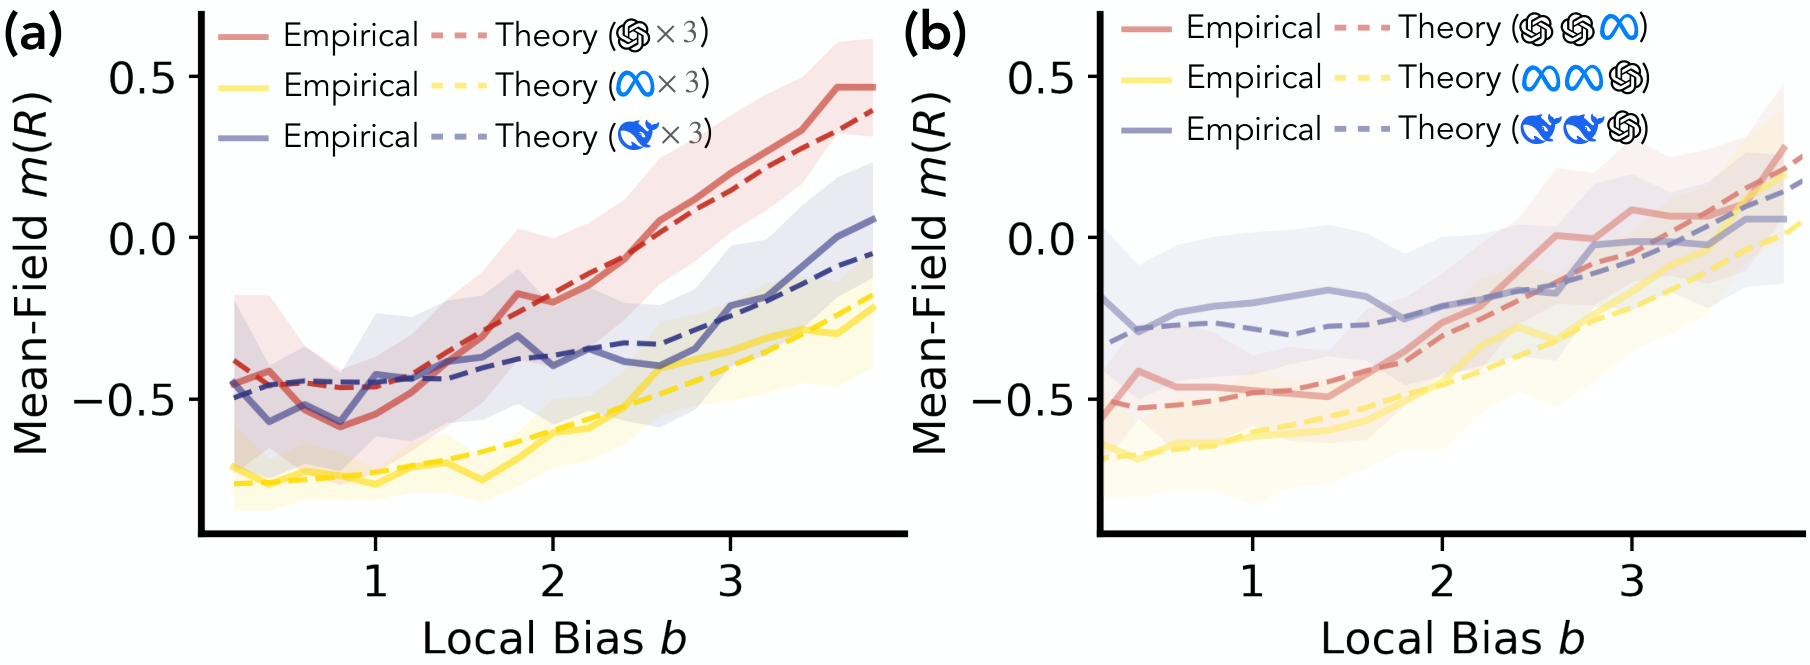
\includegraphics[width=\textwidth,height=.29\textheight,keepaspectratio]{figures/print/okawa-biased-consensus_fig2.png}
\caption{\textbf{Model heterogeneity changes susceptibility to biased consensus in this protocol.} At temperature 1.2, homogeneous and mixed three-agent groups are compared as an imposed bias varies. Mixed-group curves tend to remain closer to a mean opinion of zero, while values near $-1$ or $+1$ indicate consensus. The dashed theory curves were fitted only to homogeneous groups. This provides a concrete mechanism-level comparison; it does not establish that mixing arbitrary models always improves task quality or safety. Source: \citet{okawa-biased-consensus}, Figure 6; CC BY 4.0.}
\label{fig:atlas-okawa}
\end{figure*}
\clearpage
